\documentclass{beamer} %
\usetheme{CambridgeUS}
\usepackage[utf8]{inputenc}
\usefonttheme{professionalfonts}
\usepackage{times}
\usepackage{tikz}
\usepackage{amsmath}
\usepackage{verbatim}
\usetikzlibrary{arrows,shapes}
\setbeamertemplate{footline}[text line]{%
  \parbox{\linewidth}{\vspace*{-10pt}Universidad de Granada \hfill\hfill\insertpagenumber}}


\author{Iván Calle Gil\\ José Carlos Entrena Jiménez\\ Daniel López\\ Lothar Soto\\\textit{Universidad de Granada}}
\title{Recuperación de información \\Práctica Lucene}

\begin{document}

% For every picture that defines or uses external nodes, you'll have to
% apply the 'remember picture' style. To avoid some typing, we'll apply
% the style to all pictures.
\tikzstyle{every picture}+=[remember picture]

% By default all math in TikZ nodes are set in inline mode. Change this to
% displaystyle so that we don't get small fractions.
\everymath{\displaystyle}

\begin{frame}
\titlepage
\end{frame}

\begin{frame}
\frametitle{Introducción}
La idea inicial era hacer un programa de búsqueda desestructurada que nos permitiera obtener papers relacionados con las áreas de las matemáticas como pueden ser:
\begin{itemize}
	\item Geometría
	\item Análisis
	\item Estadística
	\item etc
\end{itemize}
De esta forma podiamos hacer una aplicación que nos facilite la búsqueda de dichos documentos cuando estemos haciendo un estudio de una determinada área.

\end{frame}

\begin{frame}
\frametitle{Colección de documentos}
Al comenzar se pretendia obtener los papers o documentos completos y hacer una aplicación para detectar una estructura en los mismos. Pero esto no es viable debido a la relación dificultad/tiempo.\\
\textbf{¿Cómo son nuestros documentos?}
\begin{itemize}
	\item Cada una de las filas de un archivo .csv.
	\item Cada archivo .csv contiene aproximadamente 2000 papers (filas).
	\item Cada fila tiene una serie de atributos.
	\item Usamos 2 algoritmos para concatenar todos los .csv y eliminar repetidos.
\end{itemize}
\end{frame}

\begin{frame}
\frametitle{Colección de documentos}
	\begin{center}
		\includegraphics[scale=0.35]{Img/Img2.png} 
	\end{center}
\end{frame}

\begin{frame}
\frametitle{Colección de documentos}
\begin{itemize}
\item De cada uno de los papers no seleccionamos todos sus atributos.
\item Se filtran los atributos para obtener aquellos que se necesitan que son los siguientes:
 \begin{itemize}
 	\item Autores
	\item Título
	\item Año
	\item Fuente (revista de publicación)
	\item Página de inicio (en la revista)
	\item Página de fin (en la revista)
	\item Enlace
	\item Abstract
	\item Palabras clave del autor
	\item Palabras clave para indexación
	\item Referencias
	\item Idioma
	\item Tipo de documento
 \end{itemize}
\end{itemize}
\end{frame}

\begin{frame}
\frametitle{Indexación}

\end{frame}

\begin{frame}
\frametitle{Vista General de la aplicación}
	\begin{center}
		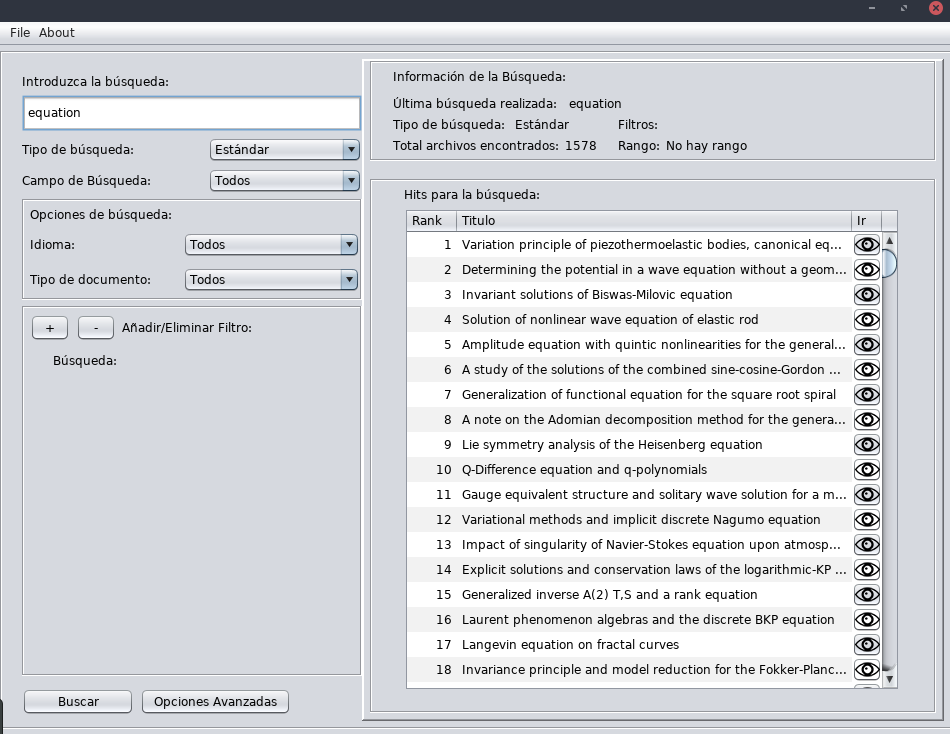
\includegraphics[scale=0.25]{Img/Img1.png} 
	\end{center}
\end{frame}

\begin{frame}
	\frametitle{Elementos de la aplicación}
	\begin{tabular}{cl}
		\begin{minipage}{0.33\textwidth}	
			\begin{center}
					\includegraphics[scale=0.35]{Img/Img3.png}
			\end{center}
		\end{minipage}
 	 & 
		\begin{minipage}[t]{0.6\textwidth}
		Construcción de búsqueda:
    	\begin{itemize}
    		\item Permite realizar la búsqueda.
    		\item Se permite pulsar enter para realizar la búsqueda
    	\end{itemize}
 	 \end{minipage}\\
		\begin{minipage}{0.33\textwidth}	
			\begin{center}
					\includegraphics[scale=0.35]{Img/Img4.png}
			\end{center}		
		\end{minipage}  
	& 
	\begin{minipage}[t]{0.6\textwidth}
	Tipo de búsqueda:
    	\begin{itemize}
    		\item Estandar: Engloba búsquedas por términos, booleana y númerica.
    		\item Proximidad: Permite realizar una búsqueda un un grado de variación o distancia.
    		\item Exacta: Búsqueda de proximidad con distancia 0.
    	\end{itemize}
 	 \end{minipage}\\
	\end{tabular} 
\end{frame}
	         
\begin{frame}
	\frametitle{Elementos de la aplicación}
	\begin{tabular}{cl}
		\begin{minipage}{0.33\textwidth}	
			\begin{center}
					\includegraphics[scale=0.35]{Img/Img5.png}
			\end{center}
		\end{minipage}
 	 & 
		\begin{minipage}[t]{0.65\textwidth}
		Campos de búsqueda:
    	\begin{itemize}
    		\item El campo Todos hace que la búsqueda se realice sobre los campos de autor, título, abstract, fuente y palabras clave.
    		\item Si este es un número también se hace sobre el año, pagina de inicio y de fin.
    	\end{itemize}
 	 \end{minipage}\\
		\begin{minipage}{0.33\textwidth}	
			\begin{center}
					\includegraphics[scale=0.35]{Img/Img6.png}
					\includegraphics[scale=0.35]{Img/Img7.png}
			\end{center}		
		\end{minipage}  
	& 
	\begin{minipage}[t]{0.65\textwidth}
	Faceta sobre el idioma:
    	\begin{itemize}
    		\item Permite filtrar el resultado por un idioma.
    		\item Obtiene la cantidad de resultados para cada idioma despues de una búsqueda.
    	\end{itemize}
 	 \end{minipage}\\
	\end{tabular} 
\end{frame}	  

\begin{frame}
	\frametitle{Elementos de la aplicación}
	\begin{tabular}{cl}
		\begin{minipage}{0.33\textwidth}	
			\begin{center}
					\includegraphics[scale=0.35]{Img/Img8.png}
			\end{center}
		\end{minipage}
 	 & 
		\begin{minipage}[t]{0.65\textwidth}
		Faceta sobre el tipo de documento:
    	\begin{itemize}
    		\item Permite filtrar el resultado por el ripo de documentos como articulos o reviews.
    		\item Al igual que con la anterior se obtiene el número de resultados despues de una búsqueda.
    	\end{itemize}
 	 \end{minipage}\\
		\begin{minipage}{0.33\textwidth}	
			\begin{center}
					\includegraphics[scale=0.35]{Img/Img9.png}
			\end{center}		
		\end{minipage}  
	& 
	\begin{minipage}[t]{0.6\textwidth}
	Añadir Filtros
    	\begin{itemize}
    		\item Añade filtros a la búsqueda por cualquier campo.
    		\item Hace uso de la búsqueda booleana para construir la nueva consulta.
    	\end{itemize}
 	 \end{minipage}\\
	\end{tabular} 
\end{frame}

\begin{frame}
	\frametitle{Elementos de la aplicación}
	\begin{center}
		\includegraphics[scale=0.45]{Img/Img10.png}
	\end{center}
	Panel de información sobre la última búsqueda realizada:
	\begin{itemize}
		\item Muestra la última búsqueda realizada.
		\item El último tipo de búsqueda realizado.
		\item El total de archivos encontrados.
		\item Si se han aplicado filtros o no y cuales son los aplicados.
		\item Si la búsqueda se ha realizado una filtración por rango o no.
	\end{itemize}		
\end{frame}

\begin{frame}
	\frametitle{Elementos de la aplicación}
	\begin{center}
		\includegraphics[scale=0.2]{Img/Img11.png}
	\end{center}
	Panel de Hits o ranking de documentos:
	\begin{itemize}
		\item Muestra un ranking con los documentos más relevantes.
		\item Se múestra el título de cada documento encontrado.
		\item Se ha añadido un icono para simplificar los enlaces directos a la web donde está alojado cada documento.
	\end{itemize}	
\end{frame}

\begin{frame}
	\frametitle{Elementos de la aplicación}
	\begin{center}
		\includegraphics[scale=0.45]{Img/Img12.png}
	\end{center}
	Panel de filtrado por rango:
	\begin{itemize}
		\item Permite filtrar por rango el resultado de la búsqueda.
		\item Puede realizarse sobre todos los campos numéricos.
		\item Se aplica igual que los filtros anteriores.
	\end{itemize}	
\end{frame}
       
\end{document}              
            